% !TEX root = frenetic_programmers_guide.tex

\chapter{Multi-Switch Topologies}
 \label{multiswitch_topologies}

Up until now, we've been working with a one-switch network.  Indeed, we can divide any SDN network into
one-switch pieces with a separate controller and network application for each.  We can even share
NIB's between these applications through a database or special network protocols.  

But this makes the SDN unncessarily complex and expensive.  By using a single controller and application
connected to a collection of switches, we gain:

\begin{itemize}
\item A simpler network application architecture.  Similar switches can share policy templates.
\item A cheaper infrastsucture by using one controller server (we can add redundant controllers if
fault tolerance is required).
\item A larger overall network view.  This eliminates the need for complex protocols like Spanning
Tree Protocol (STP).
\end{itemize}

The main thing in handling multi-switch networks is to avoid loops and broadcast storms.  These two 
problems can slow a network to a crawl.   

\section{A Simple Core/Edge Network}

Let's start with a fairly standard network topology.  

\begin{figure}[h]
\centering
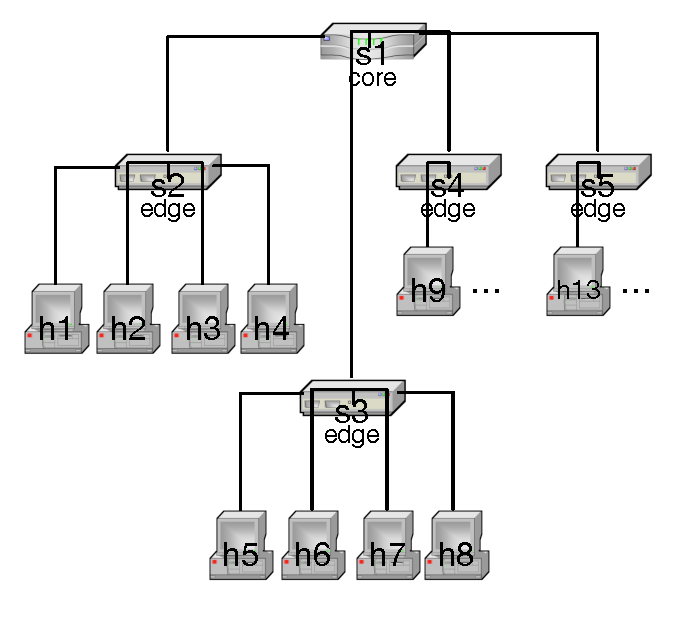
\includegraphics{switching_topo.pdf}
\end{figure}

In this network, each of the four switches s2 to s5
has four hosts of its own -- commonly one or more switches serve the hosts on a particular building floor.
These are called \emph{edge switches} because they live on the edge of the network.  Edge switches are easy to 
spot: they have end hosts connected to them.
A \emph{core switch} connects the edge switches in a bundle.  It generally doesn't have hosts
hooked up to it -- only edge switches.  

We start with the NIB from an L2 learning network and add DPID identifiers to the data
structures.  Recall the DPID, or datapath ID, uniquely identifies a switch.

The following code is in  \codefilename{multiswitch_topologies/network_information_base.py}:

\inputminted{python}{code/multiswitch_topologies/network_information_base.py}

The core switch will have different rules than the edge switches, so we need to distinguish it
from the others.  To make things easy, we hardcode the DPID of the core switch.  
In a Mininet Tree topology, the core switch always has DPID 1.  

So let's work from the edge switches inwards.  Edge switches basically learn its directly
connected hosts, like a regular L2 switch.  In fact, the NetKAT rules for the edge switch 
look like L2 rules except for the addition of \netkat{SwitchEq}.  For each learned MAC, we have a rule.

\begin{minted}{python}
Filter(SwitchEq(dpid) & EthDstEq(mac)) >> SetPort(port) 
\end{minted}

Like an L2 switch, all packets bound to/from an unlearned MAC will go the controller and get flooded
out all non-ingress ports.  The big difference, which is practically invisible in the rule, is
the packet will also go to the core switch.  That way, if the packet is bound for a host on the 
opposite side of the network, it will hop to the core switch, then to the destination switch.  

The edge switch policy is set in the application \codefilename{multiswitch_topologies/multiswitch1.py}:

\inputminted[firstline=22,lastline=40]{python}{code/multiswitch_topologies/multiswitch1.py}

And packets for unlearned MACs are handled by \python{packet_in}:

\inputminted[firstline=54,lastline=78]{python}{code/multiswitch_topologies/multiswitch1.py}

Here, we have to be a bit careful.  In a one-switch setup, we simply learn all packets coming in
on all ports.  But in a multi-switch setup, we only want to learn MACs from packets coming from
directly connected hosts.  A packet coming from a core switch comes into the \emph{uplink port}
sometimes called an \emph{internal port} because it's on an internal edge of the topology
graph.  
Such a packet represent many MACs from many hosts.  Even though those hosts may have been learned on their
ingress switches, preventing learning here, timing may cause the rules not to be installed yet.
To keep things perfectly clear, we explicitly deny learning of MAC's arriving on an internal port.

Now for the core switch.  In our first incarnation, we'll take a naive approach.  We'll make it like
a repeater -- packets coming in port $p$ will be flooded out all non-$p$ ports.  This would cause problems
in a topology with loops, but our fixed topology has no loops in it and so is safe.  The core
switch policy looks like this:

\inputminted[firstline=42,lastline=49]{python}{code/multiswitch_topologies/multiswitch1.py}

And finally because the core and edge switch policies are disjoint, we can tie them together with a 
\netkat{Union}:

\inputminted[firstline=51,lastline=52]{python}{code/multiswitch_topologies/multiswitch1.py}

We start up the Mininet topology and the Pingall pings all $16^2$ host pairs in order.  The Mininet 
topology \texttt{tree,2,4} means a tree toplogy with two levels and fanout four, meaning four
edge switches and four hosts connected to each edge switch.   

\begin{minted}{console}
frenetic@ubuntu-1404:~$ sudo mn --topo=tree,2,4 --controller=remote --mac
*** Creating network
*** Adding controller
Unable to contact the remote controller at 127.0.0.1:6633
*** Adding hosts:
h1 h2 h3 h4 h5 h6 h7 h8 h9 h10 h11 h12 h13 h14 h15 h16
*** Adding switches:
s1 s2 s3 s4 s5
*** Adding links:
(s1, s2) (s1, s3) (s1, s4) (s1, s5) (s2, h1) (s2, h2) (s2, h3) ....
*** Configuring hosts
h1 h2 h3 h4 h5 h6 h7 h8 h9 h10 h11 h12 h13 h14 h15 h16
*** Starting controller
c0
*** Starting 5 switches
s1 s2 s3 s4 s5 ...
*** Starting CLI:
mininet> pingall
*** Ping: testing ping reachability
h1 -> h2 h3 h4 h5 h6 h7 h8 h9 h10 h11 h12 h13 h14 h15 h16
h2 -> h1 h3 h4 h5 h6 h7 h8 h9 h10 h11 h12 h13 h14 h15 h16
h3 -> h1 h2 h4 h5 h6 h7 h8 h9 h10 h11 h12 h13 h14 h15 h16
h4 -> h1 h2 h3 h5 h6 h7 h8 h9 h10 h11 h12 h13 h14 h15 h16

   ... more Pings
\end{minted}

\section{Network-Wide Learning}

Out first application works, but it's pretty inefficient.  In particular:

\begin{itemize}
\item The core switch simply floods to all the switches, even when it knows (for a particular destination MAC)
where the desination switch and port is.  If it knows the egress edge switch, the core switch should send it to that switch.  
\item Packets with an unknown destination (but a known source) get flooded out the ingress switch.  
These packets come to the controller, but they don't really need to.  They could just as well be flooded 
by a switch rule.  
\end{itemize}

So let's write some rules to handle these cases.  We need to be careful not to create loops or broadcast
storms in the process.  

First we'll do the core switch.  For every destination MAC we have learned, we know its connected to
switch $sw$ at port $p$.  Actually port $p$ doesn't matter to the core switch -- it just needs to know
which core port will get it to the egress switch $sw$.  Suppose that port is $cp$.  Then the rule will look
like:

\begin{minted}{python}
Filter(SwitchEq(core) & EthDstEq(mac)) >> SetPort(cp) 
\end{minted}

First, let's factor out the port flooding policy. 
This policy will flood all packets to all other ports on the switch.  
It will be our fallback policy for all destination MACs
we don't know.  

The following code is in \codefilename{multiswitch_topologies/multiswitch2.py}:

\inputminted[firstline=22,lastline=31]{python}{code/multiswitch_topologies/multiswitch2.py}

Next, this policy constructs the learned MAC rules.  Since there's no overlap here, a simple
\netkat{Union} can be used to combine them.  (We have factored out the \netkat{SwitchEq} filter
because we'll use it for the entire switch rule.)

\inputminted[firstline=60,lastline=68]{python}{code/multiswitch_topologies/multiswitch2.py}

Finally, the entire core switch policy puts them together.  Flooding rules and learned MAC rules have
considerable overlap -- you can imagine a packet destined for a learned MAC (which matches a learned
MAC rule) which comes in a core switch port (which matches a flooding rule).  So we use \netkat{IfThenElse}
to disambiguate them.  And here we pop on the filter for the core switch, neatly factoring it out 
of the individual rules:

\inputminted[firstline=70,lastline=78]{python}{code/multiswitch_topologies/multiswitch2.py}

OK, now for the edge switches.  We basically want to refactor the rule into the following psuedocode:

\begin{minted}{python}
if unlearned(src_mac) and not internal_port(port):  
  learn(src_mac)    # Send to controller
if on_switch(dpid, dst_mac):
  send_directly()
else:
  flood()
\end{minted}

Like our previous application, we have to be careful not to learn MACs arriving on internal ports.
But here, since we're relying on the rules to do the flooding, not the controller, we have to 
explicitly filter out internal ports from the learning process with NetKAT predicates.

The new edge switch rule follows this psuedocode skeleton:

\inputminted[firstline=39,lastline=52]{python}{code/multiswitch_topologies/multiswitch2.py}

The remaining code stays the same.  Now doing a Ping All in Mininet is a much faster experience -- once all the
ports are learned (h1 pings each host in turn first, so that does the learning), no packets hit the controller.
Very nice!

\begin{quotation}
\emph{NOTE:  ARP doesn't work very well with this, but it's unclear why.  h1 sends an ARP request for
h2, \ldots but it's unclear whether the request is flooded properly by the controller, or whether the
reply comes back.  This is true for all hosts, intranet or internet.  But once the flow table is complete,
everything works fine including (presumably) ARP requests.   Use the arp command switch in Mininet 
and the problem doesn't happen at all.   }
\end{quotation}


\section{Calculating Loop-Free Paths}

To get to this point, we've had to effectively hard-code the network topology into the program.  The next step
is to extend it to work with \emph{any} topology.  

The basic problem is: given two host endpoints and a topology, what is the shortest path through the switches 
connecting those hosts?  Once you have that, you can generate a rule for each switch -- basically the 
rule will forward packets one hop closer to the destination.  In effect, our first programs hard-coded the shortest
path solutions because they were trivial for that topology:

\begin{itemize}
\item If the destination is on the same switch as the source, just forward it out the right port.
\item If it's not, forward it to the core switch, then to the destination edge switch, then out the right port.
\end{itemize}

If you had never worked with computer networks you'd think we could stop there.  Computing shortest paths
is an easy graph theoretical problem, and we could just have a library do it.  Not only that, you could
just connect every switch to every other switch, and the number of hops between any two hosts would be 
two.  

The only trouble is \ldots there is flooding.  If every switch is connected to every switch, and you copy
a packet to all the ports at once, it'll eventually arrive back at the source switch and get flooded again
and again.  This is called a \emph{broadcast storm} and it'll eventually grind the network to a halt.  
And you can't just get rid of flooding.  Even if get rid of Ethernet broadcasts, flooding is a major part
of L2 learning -- it's how you deal with packets going to as-yet-unlearned destinations.

One way to have total connectivity without loops is to calculate the \emph{spanning tree} of the topology.
In a spanning tree, all switches are indirectly connected by some path, but the total collection of
paths contains no loops.  As long as flooding occurs only along the paths of the spanning tree (and
not out the ingress port too, of course), no broadcast storms are possible.   This spanning tree
might not be optimal in a shortest path sense -- it might force some host-to-host paths to be longer than 
they could be.  But the added safety is well-worth the cost.  

Traditional Ethernet networks use a protocol like STP to cooperatively decide on the spanning tree.  STP is 
interesting but it's complex and slow to converge.  The problem is no one switch has a total view of the 
network -- it only knows its neighbors.  

SDN doesn't have that problem.  The controller effectively can use a
global view of the network, from which it calculates the spanning tree and pushes the resulting rules to all
the switches at once.  

But how does it get that global view of the topology, especially when switches can dynamically enter and leave the
network?  Let's defer that question for now, and focus on a fixed toplogy but one that can be
defined outside of the program itself.  Once we build the infrastructure that calculates the spanning tree
and forwarding rules from this topology, we can generalize it to dynamic toplogies.  

There are many different file formats for specifying a network topology.  We're going to use the popular
\emph{GraphViz} file format.  GraphViz files can be read from lots of different programming languages, and can easily
be turned into visible graphs.  In Python, it's also easy to interface GraphViz files with the popular 
graph theory library NetworkX.  We can then leverage NetworkX's spanning tree and shortest-path 
algorithms rather than writing our own.  Nice!

To make this topology more interesting, we're going to use a Mininet tree topology with depth 3 and fanout 3.
That'll give us 1 at the top level, three at the second level, and nine at the third level
for a total of $1 + 3 + 9 = 13$ switches and three hosts connected to the 9 level 3 switches, for a total of 27
hosts:

\begin{minted}{console}
frenetic@ubuntu-1404:~$ sudo mn --topo=tree,3,3 --controller=remote --mac
*** Creating network
*** Adding controller
Unable to contact the remote controller at 127.0.0.1:6633
*** Adding hosts:
h1 h2 h3 h4 h5 h6 h7 h8 h9 h10 h11 h12 h13 h14 h15 h16 h17 h18 h19 h20 h21 h22 h23 h24 h25 h26 h27
*** Adding switches:
s1 s2 s3 s4 s5 s6 s7 s8 s9 s10 s11 s12 s13
*** Adding links:
(s1, s2) (s1, s6) (s1, s10) (s2, s3) (s2, s4) (s2, s5) (s3, h1) (s3, h2) (s3, h3) (s4, h4) 
(s4, h5) (s4, h6) (s5, h7) (s5, h8) (s5, h9) (s6, s7) (s6, s8) (s6, s9) (s7, h10) (s7, h11) 
(s7, h12) (s8, h13) (s8, h14) (s8, h15) (s9, h16) (s9, h17) (s9, h18) (s10, s11) (s10, s12) 
(s10, s13) (s11, h19) (s11, h20) (s11, h21) (s12, h22) (s12, h23) (s12, h24) (s13, h25) 
(s13, h26) (s13, h27)
*** Configuring hosts
h1 h2 h3 h4 h5 h6 h7 h8 h9 h10 h11 h12 h13 h14 h15 h16 h17 h18 h19 h20 h21 h22 h23 h24 h25 h26 h27
*** Starting controller
c0
*** Starting 13 switches
s1 s2 s3 s4 s5 s6 s7 s8 s9 s10 s11 s12 s13 ...
*** Starting CLI:
mininet>
\end{minted} 

Now the Mininet tree toplogy has no loops, but we can add one on the sly:

\begin{minted}{console}
mininet> py net.addLink(s2, s6) 
<mininet.link.Link object at 0x7fd432ace810>
mininet> link s2 s6 up
mininet> py s2.attach('s2-eth5')
\end{minted}

Next we write a GraphViz file that mirrors this topology, including the extra edge.  
So here is our DOT file, from \codefilename{multiswitch_topologies/multiswitch_topo.dot}:

\inputminted{python}{code/multiswitch_topologies/multiswitch_topo.dot}

This file is pretty straightforward to read:

\begin{itemize}
\item The switches are listed by themselves first.  We'll keep it simple and name each one after the DPID that
Mininet will naturally assign to it: e.g. s13 will have DPID 13.
\item The edges are listed next, each edge being a pair of switches separated by two dashes.
\item Each edge has two attributes: \python{src_port} is the port used on the first switch and \python{dport}
is the port on the second switch.  
\end{itemize}

And you can turn this into a PDF-formatted graph with the command:

\begin{minted}{console}
dot -Tpdf multiswitch_topo.dot -o multiswitch_topo.pdf
\end{minted}

Which looks like this:

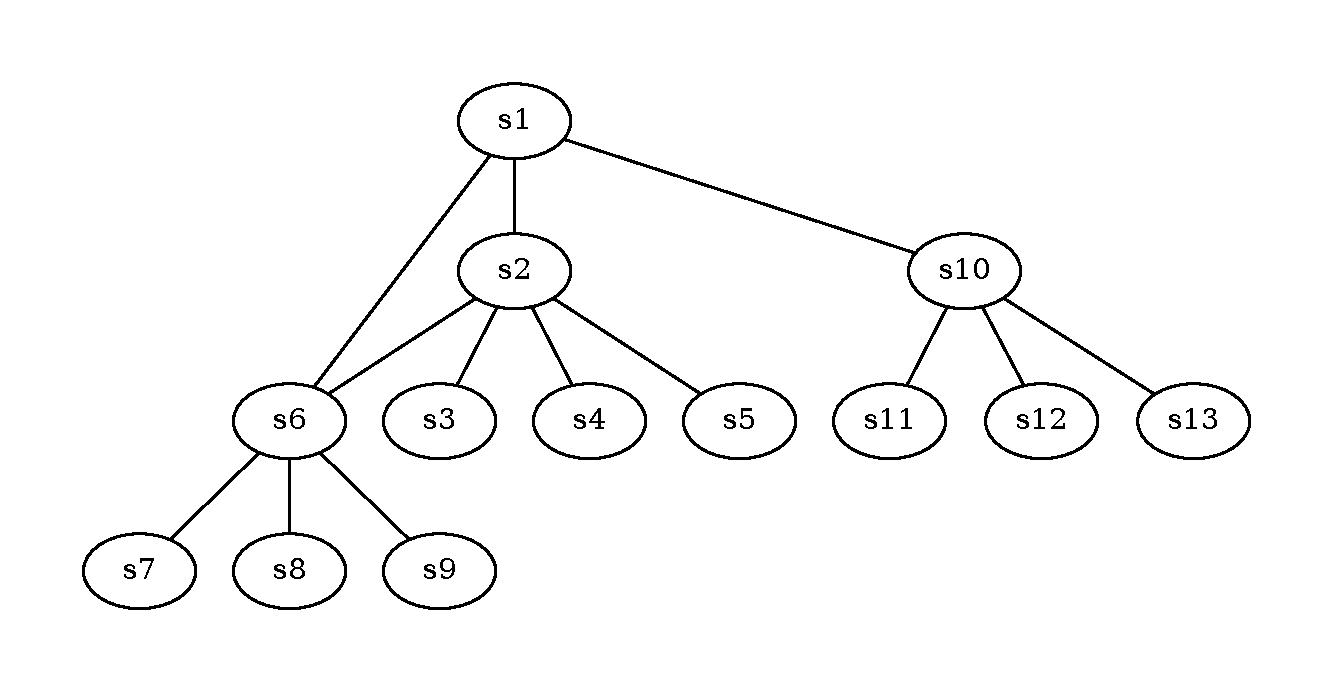
\includegraphics[width=\linewidth]{multiswitch_topo.pdf}

You can see the loop s1-s2-s6 here.

For the code, we'll start with the NIB.  We'll still keep the distinction between core and edge switches:
the edge switches being where hosts are connected, and core switches being those on the internal
portion fo the network.  Only this time we'll leave these sets blank and fill them in from the topology.

The following code is in  \codefilename{multiswitch_topologies/network_information_base_from_file.py}:

\inputminted[firstline=15,lastline=16]{python}{code/multiswitch_topologies/network_information_base_from_file.py}

Next we build a data structure for holding the direct connections between hosts and switches, or
between switches and switches.  This is a dictionary whose keys are MAC addresses for hosts and DPID's for
switches (there is no overlap between the two).  The value for each key is itself a dictionary of destinations
reachable from that source (the keys are, again, MAC addresses and DPID's), and the port they go out on.
Each host is assumed to have one switch connection on port 0, although this is really a placeholder because a host is not
a switch and therefore has no rules of its own: it can only send packets to its connected switch.  

\inputminted[firstline=21,lastline=27]{python}{code/multiswitch_topologies/network_information_base_from_file.py}

Note that this data is separate from the spanning tree, so just because we have a direct connection from one
host/switch to another doesn't mean we'll actually use it!

The \python{ports} data structure is the same one we've used in previous network applications, but
we need a parallel structure to track \emph{enabled} ports.  When we calculate the spanning tree, it's
possible that some core switch ports need to be virtually disabled because they form 
redundant paths.  For example, in our network, the edge s2-s6 is not needed in the spanning tree, and so the ports
for that edge (port 5 on s2 and port 5 on s6) will need to be virtually disabled - no floodable traffic
will go that port, and all packets arriving on that port (there shouldn't be any, but you never know) will
be dropped.

\inputminted[firstline=29,lastline=33]{python}{code/multiswitch_topologies/network_information_base_from_file.py}

The uplink port on each of the edge switches needs to be calculated and tracked, since MAC learning cannot
occur on that port.

\inputminted[firstline=18,lastline=19]{python}{code/multiswitch_topologies/network_information_base_from_file.py}

The \python{init} function is more involved, reading the topology from our DOT file and building the 
intermediate data structures.

\inputminted[firstline=40,lastline=94]{python}{code/multiswitch_topologies/network_information_base_from_file.py}

The \python{minimum_spanning_tree} method 
calculates the minimal spanning tree for the topology (minimal meaning using the least cost, and
in our case all edges have cost 1).  Then we calculate all the enabled ports whose edges live on this
spanning tree.  We print the spanning tree to the log for reference:

\begin{minted}{console}
frenetic@ubuntu-1404:~/manual/programmers_guide/code/multiswitch_topologies$ python multiswitch3.py
2016-05-27 14:49:11,162 [INFO] ---> Reading Topology from multiswitch_topo.dot
2016-05-27 14:49:11,163 [INFO] ---> Remembering internal ports
2016-05-27 14:49:11,164 [INFO] ---> Calculating spanning tree
11 10 {'dport': u'4', 'src_port': u'1'}
10 1 {'dport': u'4', 'src_port': u'3'}
10 13 {'dport': u'4', 'src_port': u'3'}
10 12 {'dport': u'4', 'src_port': u'2'}
1 2 {'dport': u'4', 'src_port': u'1'}
1 6 {'dport': u'4', 'src_port': u'2'}
3 2 {'dport': u'4', 'src_port': u'1'}
2 5 {'dport': u'4', 'src_port': u'3'}
2 4 {'dport': u'4', 'src_port': u'2'}
7 6 {'dport': u'4', 'src_port': u'1'}
6 8 {'dport': u'4', 'src_port': u'2'}
6 9 {'dport': u'4', 'src_port': u'3'}
Starting the tornado event loop (does not return).
\end{minted}

Note that the edges from s1-s2 and s1-s6 are present, but the edge s2-s6 is not listed.  It has been 
dropped calcuating the minimal spanning tree.  This final topology graph now has no loops.

This basic graph won't change.  When we connect hosts to the edge switches, it doesn't change the 
spanning tree because hosts only add one edge to the graph.  That edge must be part of the spanning tree
in order to reach the new host, but it cannot form a loop because the rest of the graph has no loops
and the new host was previously unconnected.  

Knowing all this, we can redo the MAC learning function:

\inputminted[firstline=116,lastline=148]{python}{code/multiswitch_topologies/network_information_base_from_file.py}

The main addition is the \python{next_hop} dictionary to the MAC.   This dictionary basically tells you how to
go from any switch to this MAC.  Knowing this, you can easily trace a path from any source host through as set
of switches, and finally to this destination MAC.  The path is guaranteed not to have any loops no matter
which switch you start from.  

A set of utility functions gathers important information for calculating the switch 
forwarding rules:

\inputminted[firstline=95,lastline=115]{python}{code/multiswitch_topologies/network_information_base_from_file.py}

And a new function returns the enabled ports for a particular switch, so rational flooding can occur.
This is important for the core switches.  The edge switches merely flood to all ports since the host ports
and the uplink ports are always part of the spanning tree.   

\inputminted[firstline=194,lastline=196]{python}{code/multiswitch_topologies/network_information_base_from_file.py}

Our new learning switch program won't change much.  It'll delegate most of the complex stuff to the 
NIB, which has precalculated all the routes for us.  

The following code is in \codefilename{multiswitch_topologies/multiswitch3.py}:

\inputminted[firstline=60,lastline=68]{python}{code/multiswitch_topologies/multiswitch3.py}

In this example, the core switch rule calculation has been delegated to the \python{next_hop} calculations in
the NIB.  

The flooding policy for edge switches doesn't change because each edge switch has only hosts (which must
receive the flooded packets) and one uplink port (which also must receive the flooded packet), modulo the
ingress port as always.  Core switch flooding, however, must respect the spanning tree so as not to
introduce loops:

\inputminted[firstline=22,lastline=24]{python}{code/multiswitch_topologies/multiswitch3.py}

And with that, our network keeps itself loop-free and functional.  If the topology changes, we simply
change the GraphViz file and restart that network application, which then recalculates the spanning
tree and relearns the host MAC addresses.  One can build a very large L2 network with lots of 
switches connected arbitrarily in this manner.  And it's fairly easy to extend this program for fault
tolerance -- if a port on a core switch goes down, we can update the graph, recalculate the spanning
tree, enable previously-disabled ports and keep the network running smoothly.  

\section{Summary}

To handle multiple switches, the most important thing is to avoid loops.  Taking advantage of a global network
view, we can construct loop-free paths from any host to any other host, then encode the paths in switch rules.

Note that the switch rule tables can be pretty large for large networks.  We can make them somewhat smaller 
by segmenting our network into VLANs and using the techniques in chapter 5.  This way the source/destination pairs
are constrained by the VLANs themselves.  

Our techniques have used fixed networks, but what if we want to create a dynamic network, where we can add and remove
switches at will?  This is possible through a topology discovery module.  There's a sample Frenetic net app written
in Python in \codefilename{lang/python/frenetic/examples/discovery} which does this.

All of the net apps we've written so far have ignored TCP/IP packet headers.  But this information is useful
for emulating other network devices like routers, so we'll take that up in the next chapter.  